\documentclass[a4paper]{article}
\usepackage[utf8]{inputenc}
\usepackage[russian,english]{babel}
\usepackage[T2A]{fontenc}
\usepackage[left=10mm, top=20mm, right=18mm, bottom=15mm, footskip=10mm]{geometry}
\usepackage{indentfirst}
\usepackage{amsmath,amssymb}
\usepackage{mathastext} 
\usepackage[italicdiff]{physics}
\usepackage{graphicx}
\usepackage{caption}
\usepackage{float}
\usepackage{caption}
\renewcommand{\thefootnote}{\fnsymbol{footnote}}
\usepackage{tablefootnote}
\usepackage{footmisc}
\usepackage{textcomp}
\usepackage{multicol}
\usepackage{multirow}
\usepackage[parfill]{parskip}
\usepackage{makecell}
\usepackage{array}  
\usepackage{siunitx}
\usepackage{booktabs}
\sisetup{
    exponent-product = \cdot,
    per-mode = symbol,
    separate-uncertainty = true,
    uncertainty-separator = \,
}
\renewcommand\cellalign{cc} 
\renewcommand\cellgape{\Gape[2pt]} 
\usepackage[utf8]{inputenc}\newcommand{\approxtext}[1]{\ensuremath{\stackrel{\text{#1}}{\approx}}}
\usepackage[colorlinks=true, urlcolor=blue, linkcolor=blue, citecolor=blue]{hyperref}
\graphicspath{{images/}}
\DeclareGraphicsExtensions{.pdf,.png,.jpg}
\usepackage{wrapfig}
\captionsetup{labelformat=empty}
\usepackage{caption}
\captionsetup[figure]{name=Рисунок}
\captionsetup[table]{name=Таблица}
%\usepackage{newtxtext,newtxmath} 
\title{\textbf{Отчет о выполнении лабораторной работы 3.4.1}}
\date{}
\author{Котляров Михаил, Б01-402}

\begin{document}

\maketitle
	
\section*{Введение}

\subsection*{Цель работы}
Измерение магнитной восприимчивости диа- и парамагнитных образцов методом Гюи.

\subsection*{Оборудование}
\begin{itemize}
    \item Электромагнит с регулируемым источником постоянного тока
    \item Аналитические весы
    \item Милливеберметр
    \item Образцы: медь, алюминий, графит, вольфрам
    \item Измерительные пробные катушки
\end{itemize}

\subsection*{Теоретическая часть}
Магнитная восприимчивость тел определяется по измерению сил, действующих на тела в магнитном поле. В методе Гюи используется тонкий длинный стержень, один конец которого помещают в зазор электромагнита, а другой --- вне зазора.

Сила, действующая на цилиндрический образец в магнитном поле, определяется выражением:
\[
F_M = \chi \frac{B_0^2}{2\mu_0} S
\]
где:
\begin{itemize}
    \item $\chi$ --- магнитная восприимчивость образца
    \item $B_0$ --- магнитная индукция в зазоре электромагнита
    \item $\mu_0 = 4\pi \cdot 10^{-7}$ Гн/м --- магнитная постоянная
    \item $S$ --- площадь поперечного сечения образца
\end{itemize}

Парамагнетики ($\chi > 0$) вталкиваются в зазор электромагнита, диамагнетики ($\chi < 0$) выталкиваются из него.
\clearpage
\subsection*{Экспериментальная установка}

\begin{figure}[h]
    \centering
    
\includegraphics[scale=0.6]{Pictures/ustanovka.png}
    \caption{Схема экспериментальной установки}
\end{figure}


Установка состоит из электромагнита с полюсами большого диаметра, создающего магнитное поле до 1 Тл в зазоре. Образцы поочерёдно подвешиваются к аналитическим весам так, что один конец находится в зазоре электромагнита, а другой --- вне его. Магнитное поле измеряется с помощью милливеберметра или датчика Холла.



\section*{Ход работы}

\begin{enumerate}
    \item Проверим работу цепи питания электромагнита и оценим диапазон изменения тока через обмотки.
    
    \item Прокалибруем электромагнит. С помощью милливеберметра измерим зависимость магнитного потока $\Phi$ от тока $I$ через обмотки электромагнита. Рассчитаем магнитную индукцию по формуле $B = \frac{\Phi}{SN}$, где $SN = 72 \text{ см}^2$ --- постоянная пробной катушки. Построим градуировочную кривую электромагнита $B(I) = k \cdot I + b$.

\begin{figure}[h]
    \centering
    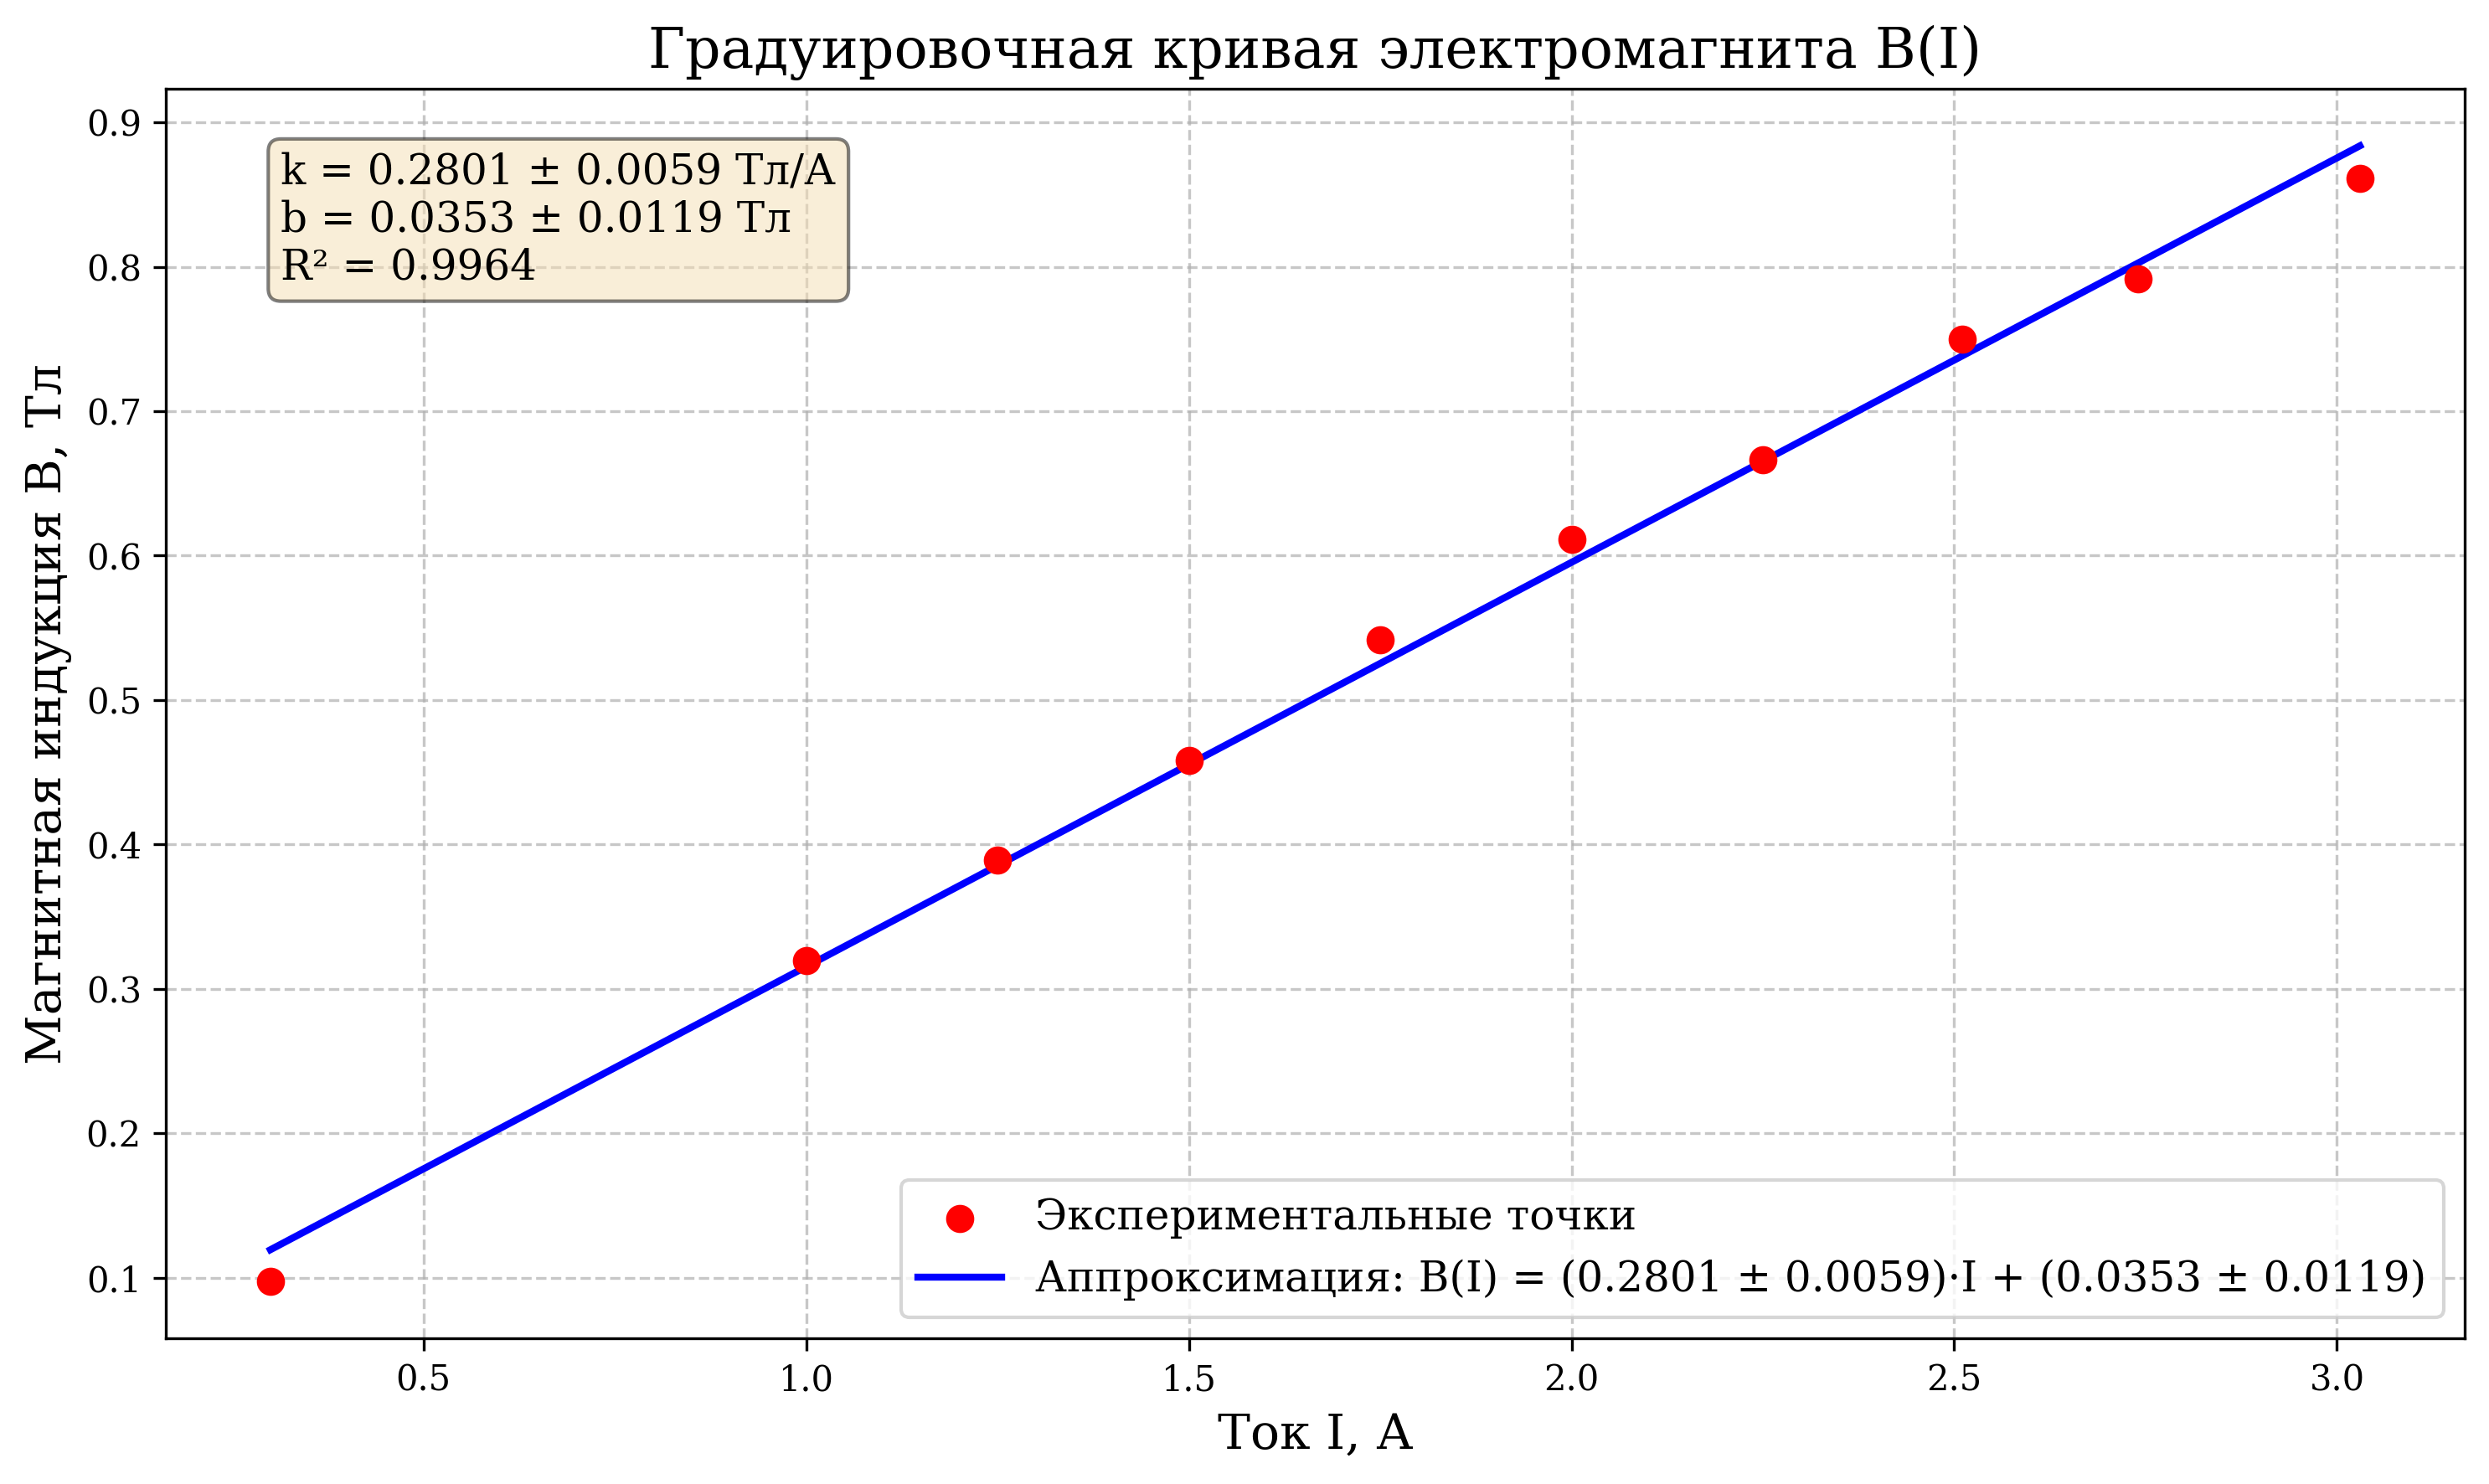
\includegraphics[scale=0.6]{Graphics/градуировочная_кривая_B(I).png}
    \caption{График 1. Градуировочную кривую электромагнита $B(I)$}
\end{figure}

\clearpage
\begin{table}[h!]
    \centering
    \begin{tabular}{|c|c|c|}
        \hline
        $I$, А & $\Delta \Phi$, мВб & $B$, Тл \\ \hline
        0,30 & 0,70 & 0,097 \\ \hline
        1,00 & 2,30 & 0,319 \\ \hline
        1,25 & 2,80 & 0,389 \\ \hline
        1,50 & 3,30 & 0,458 \\ \hline
        1,75 & 3,90 & 0,542 \\ \hline
        2,00 & 4,40 & 0,611 \\ \hline
        2,25 & 4,80 & 0,667 \\ \hline
        2,51 & 5,40 & 0,750 \\ \hline
        2,74 & 5,70 & 0,792 \\ \hline
        3,03 & 6,20 & 0,861 \\ \hline
    \end{tabular}
    \caption{Результаты калибровки электромагнита}
    \label{tab:calibration}
\end{table}


    
Параметры кривой: $k = 0,2801 \pm 0,0059 \ \frac{\text{Тл}}{\text{А}} \ (\varepsilon_k = 2,11 \%)$, $b = 0,0353 \pm 0,0119 \ (\varepsilon_b = 33,71 \%)$.

    \item Убедимся, что механические весы агрегированы. Проведём агрегирование перед каждым изменением тока.
    
    \item Измерим силы, действующие на образцы в магнитном поле. Для каждого образца:
    \begin{itemize}
        \item Подвесим образец к весам при выключенном электромагните
        \item Установим примерное значение массы образца и добьёмся точного равновесия
        \item Агрегируем весы
        \item Установим минимальное значение тока и измерим равновесное значение массы
        \item Повторим измерения для 8-10 значений тока
    \end{itemize}
    
    \item Для каждого материала построим график зависимости $|\Delta P| = f(B^2)$.
    
    \item По наклону полученных прямых рассчитаем магнитную восприимчивость $\chi$ по формуле:
    \[
    \chi = \frac{2\mu_0 k}{S}
    \]
    где $k$ --- коэффициент наклона графика $|\Delta P|(B^2)$.
    
    \item Оценим погрешности измерений и сравним экспериментальные результаты с табличными значениями.


\begin{table}[h!]
    \centering
    \begin{minipage}{0.48\textwidth}
        \centering
        \begin{tabular}{|c|c|c|c|}
            \hline
            $I$, А & $B^2 \pm \sigma_{B^2}$, Тл$^2$ & $\varepsilon_{B^2}$, \% & $|\Delta P|$, $10^{-5}$ Н \\ \hline
        1,01 & $0,1013 \pm 0,0027$ & 2,66 & 1,98 \\ \hline
        1,09 & $0,1160 \pm 0,0031$ & 2,71 & 2,97 \\ \hline
        1,24 & $0,1464 \pm 0,0041$ & 2,79 & 3,96 \\ \hline
        1,50 & $0,2074 \pm 0,0062$ & 2,97 & 5,94 \\ \hline
        1,75 & $0,2761 \pm 0,0087$ & 3,15 & 7,93 \\ \hline
        2,01 & $0,3580 \pm 0,0120$ & 3,36 & 10,9 \\ \hline
        2,26 & $0,4467 \pm 0,0160$ & 3,57 & 12,9 \\ \hline
        2,51 & $0,5452 \pm 0,0207$ & 3,80 & 15,9 \\ \hline
        2,75 & $0,6490 \pm 0,0261$ & 4,02 & 17,8 \\ \hline
        3,00 & $0,7667 \pm 0,0327$ & 4,27 & 20,8 \\ \hline
        \end{tabular}
        \caption{Медь ($d = 1$ см)}
        \label{tab:copper}
    \end{minipage}
    \hfill
    \begin{minipage}{0.48\textwidth}
        \centering
        \begin{tabular}{|c|c|c|c|}
            \hline
            $I$, А & $B^2 \pm \sigma_{B^2}$, Тл$^2$ & $\varepsilon_{B^2}$, \% & $|\Delta P|$, $10^{-5}$ Н \\ \hline
        0,75 & $0,06021 \pm 0,00153$ & 2,54 & 3,96 \\ \hline
        1,00 & $0,09948 \pm 0,00264$ & 2,66 & 5,94 \\ \hline
        1,25 & $0,1486 \pm 0,0042$ & 2,80 & 9,91 \\ \hline
        1,50 & $0,2074 \pm 0,0062$ & 2,97 & 13,9 \\ \hline
        1,75 & $0,2761 \pm 0,0087$ & 3,15 & 17,8 \\ \hline
        2,00 & $0,3546 \pm 0,0119$ & 3,35 & 22,8 \\ \hline
        2,25 & $0,4429 \pm 0,0158$ & 3,57 & 28,7 \\ \hline
        2,50 & $0,5410 \pm 0,0205$ & 3,79 & 34,7 \\ \hline
        2,76 & $0,6535 \pm 0,0264$ & 4,03 & 40,6 \\ \hline
        3,03 & $0,7815 \pm 0,0336$ & 4,30 & 46,6 \\ \hline
        \end{tabular}
        \caption{Алюминий ($d = 1$ см)}
        \label{tab:aluminum}
    \end{minipage}
\end{table}

\begin{table}[h!]
    \centering
    \begin{minipage}{0.48\textwidth}
        \centering
        \begin{tabular}{|c|c|c|c|}
            \hline
            $I$, А & $B^2 \pm \sigma_{B^2}$, Тл$^2$ & $\varepsilon_{B^2}$, \% & $|\Delta P|$, $10^{-5}$ Н \\ \hline
        0,65 & $0,04725 \pm 0,00118$ & 2,50 & 1,98 \\ \hline
        1,00 & $0,09948 \pm 0,00264$ & 2,66 & 5,94 \\ \hline
        1,25 & $0,1486 \pm 0,0042$ & 2,80 & 8,92 \\ \hline
        1,50 & $0,2074 \pm 0,0062$ & 2,97 & 13,9 \\ \hline
        1,75 & $0,2761 \pm 0,0087$ & 3,15 & 18,8 \\ \hline
        1,99 & $0,3513 \pm 0,0118$ & 3,34 & 23,8 \\ \hline
        2,25 & $0,4429 \pm 0,0158$ & 3,57 & 30,7 \\ \hline
        2,50 & $0,5410 \pm 0,0205$ & 3,79 & 37,6 \\ \hline
        2,75 & $0,6490 \pm 0,0261$ & 4,02 & 44,6 \\ \hline
        3,00 & $0,7667 \pm 0,0327$ & 4,27 & 50,5 \\ \hline
        \end{tabular}
        \caption{Графит ($d = 0,56$ см)}
        \label{tab:graphite}
    \end{minipage}
    \hfill
    \begin{minipage}{0.48\textwidth}
        \centering
        \begin{tabular}{|c|c|c|c|}
            \hline
            $I$, А & $B^2 \pm \sigma_{B^2}$, Тл$^2$ & $\varepsilon_{B^2}$, \% & $|\Delta P|$, $10^{-4}$ Н \\ \hline
        0,50 & $0,03075 \pm 0,00075$ & 2,45 & 0,495 \\ \hline
        0,75 & $0,06021 \pm 0,00153$ & 2,54 & 1,19 \\ \hline
        0,99 & $0,09772 \pm 0,00259$ & 2,65 & 2,18 \\ \hline
        1,26 & $0,1507 \pm 0,0042$ & 2,81 & 3,37 \\ \hline
        1,50 & $0,2074 \pm 0,0062$ & 2,97 & 4,76 \\ \hline
        1,75 & $0,2761 \pm 0,0087$ & 3,15 & 6,54 \\ \hline
        2,00 & $0,3546 \pm 0,0119$ & 3,35 & 8,32 \\ \hline
        2,25 & $0,4429 \pm 0,0158$ & 3,57 & 10,3 \\ \hline
        2,50 & $0,5410 \pm 0,0205$ & 3,79 & 12,3 \\ \hline
        2,75 & $0,6490 \pm 0,0261$ & 4,02 & 14,4 \\ \hline
        3,00 & $0,7667 \pm 0,0327$ & 4,27 & 16,3 \\ \hline
        \end{tabular}
        \caption{Вольфрам ($d = 1$ см)}
        \label{tab:tungsten}
    \end{minipage}
\end{table}



\begin{figure}[h]
    \centering
    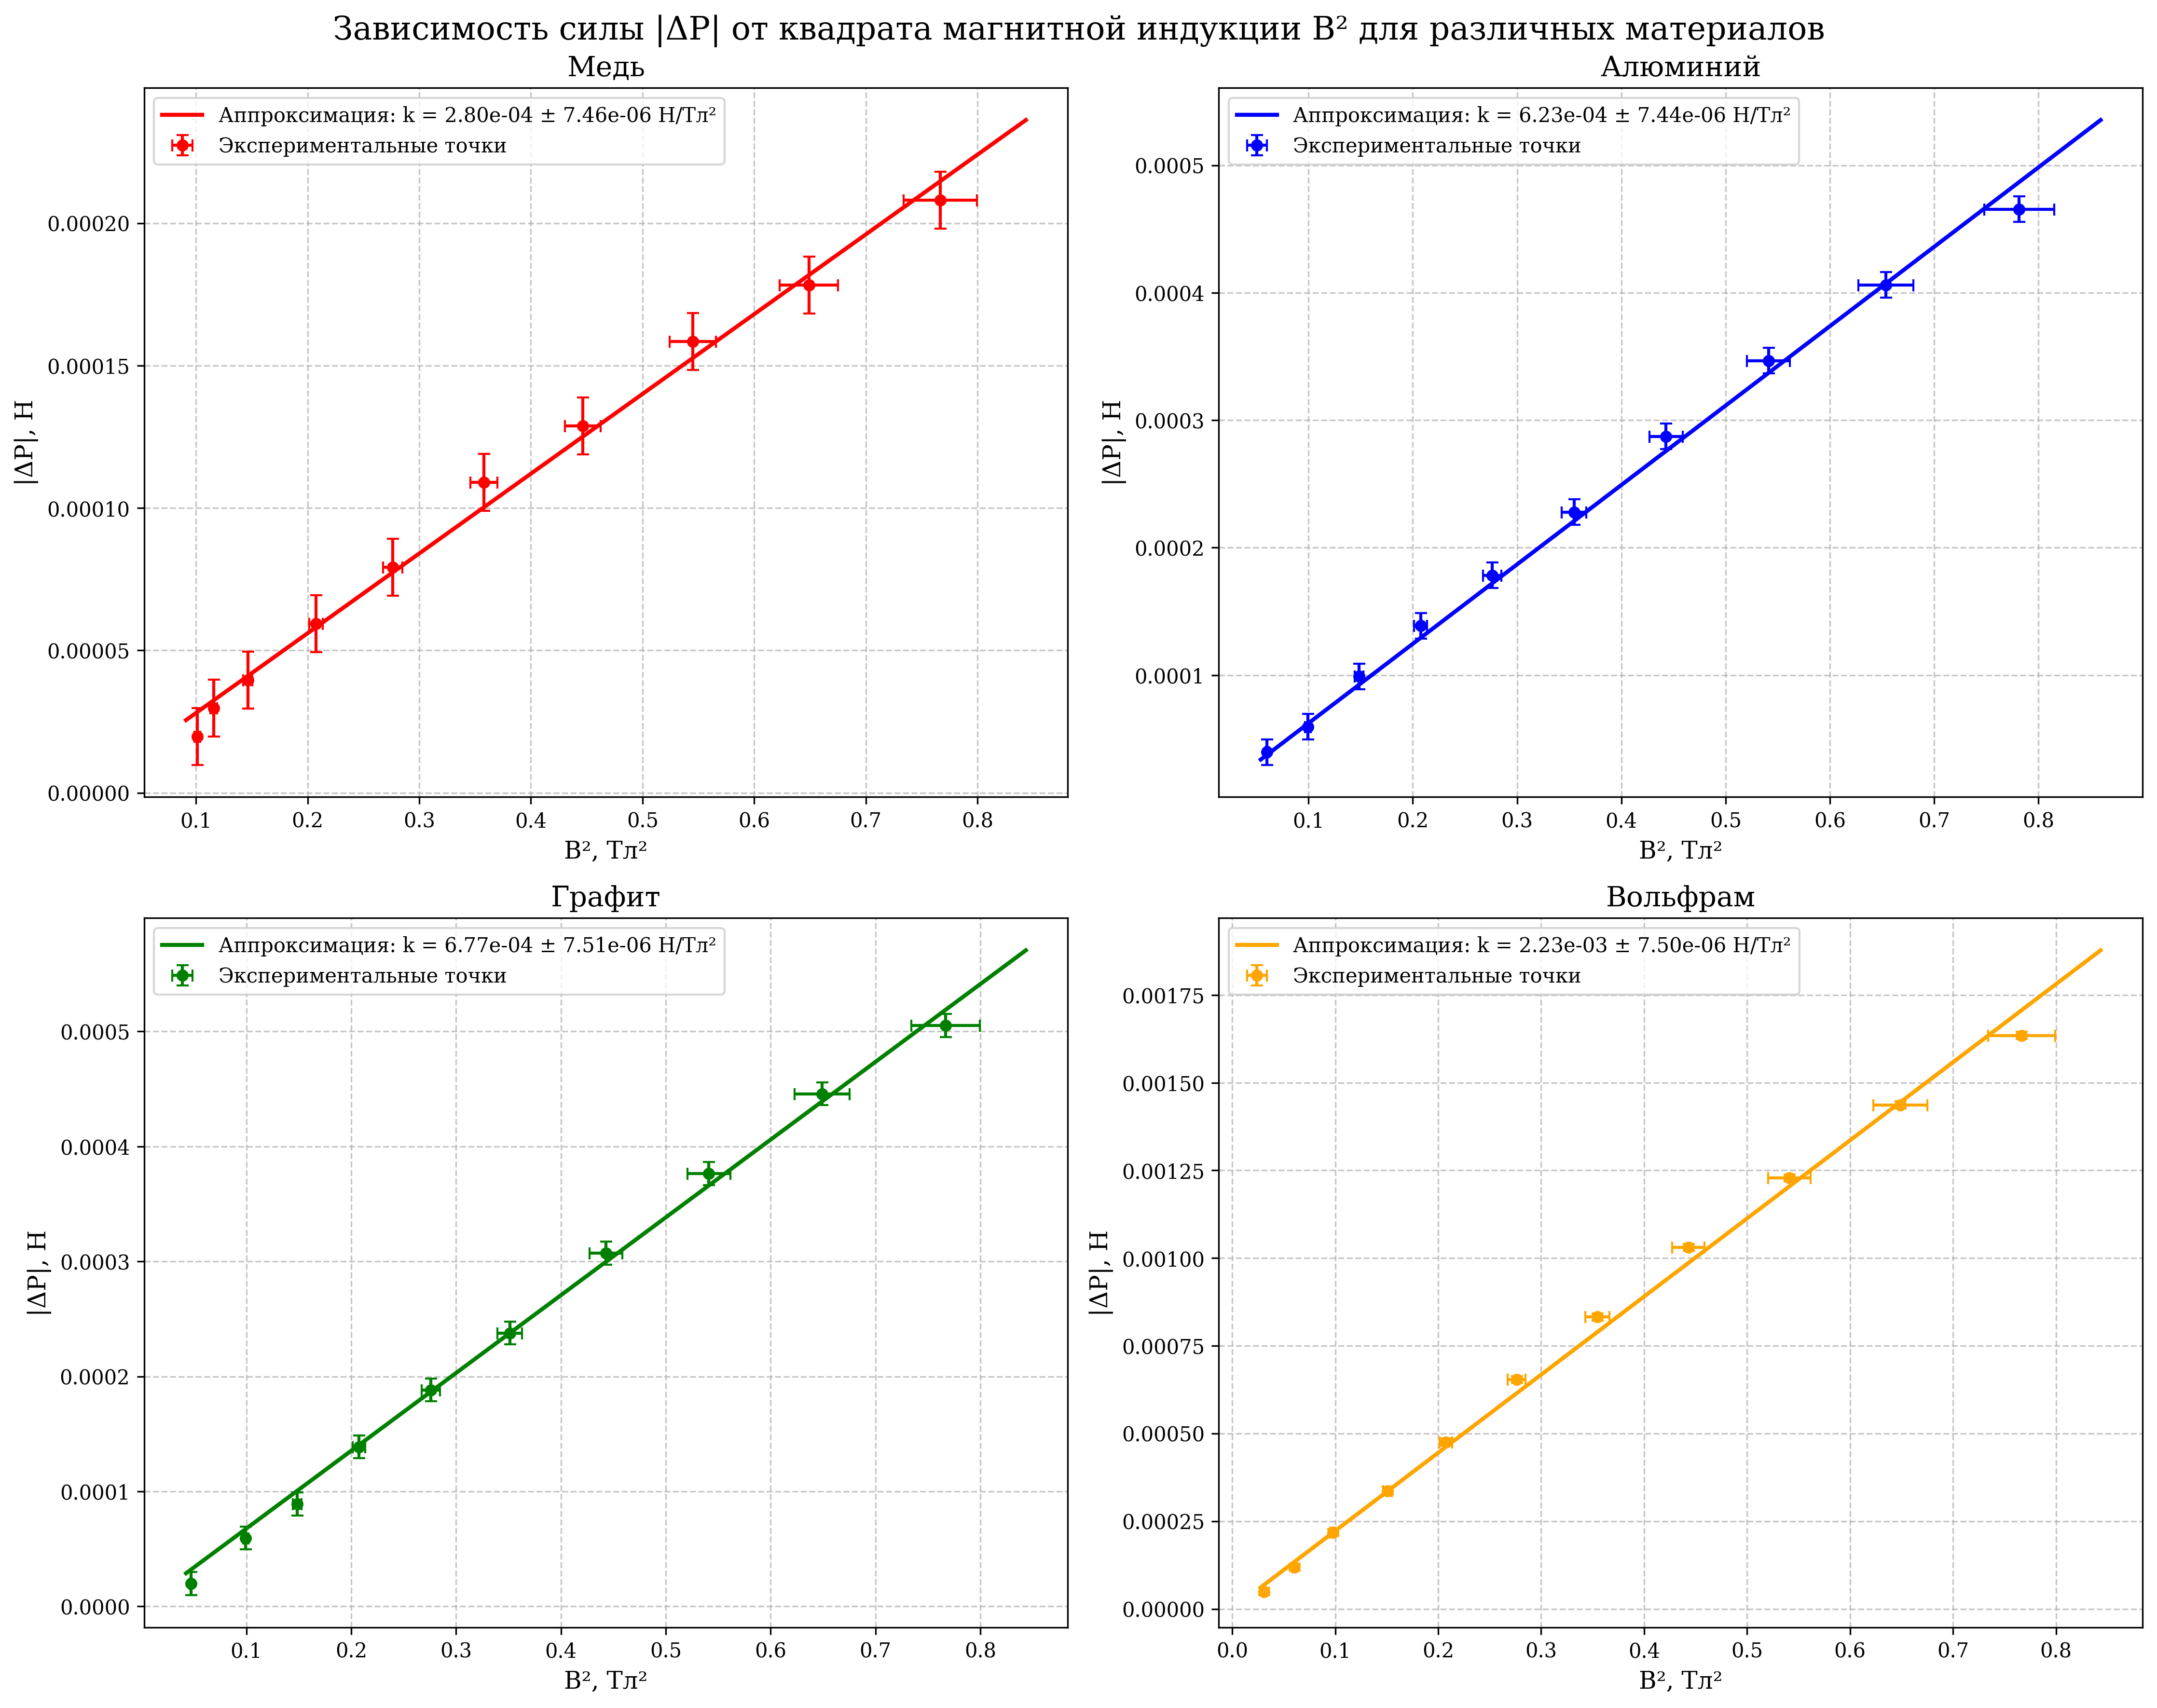
\includegraphics[scale=0.5]{Graphics/all_materials_separate.png}
    \caption{График 2. Графики зависимостей $|\Delta P|(B^2)$ для разных материалов.}
\end{figure}
\clearpage
\begin{figure}[h]
    \centering
    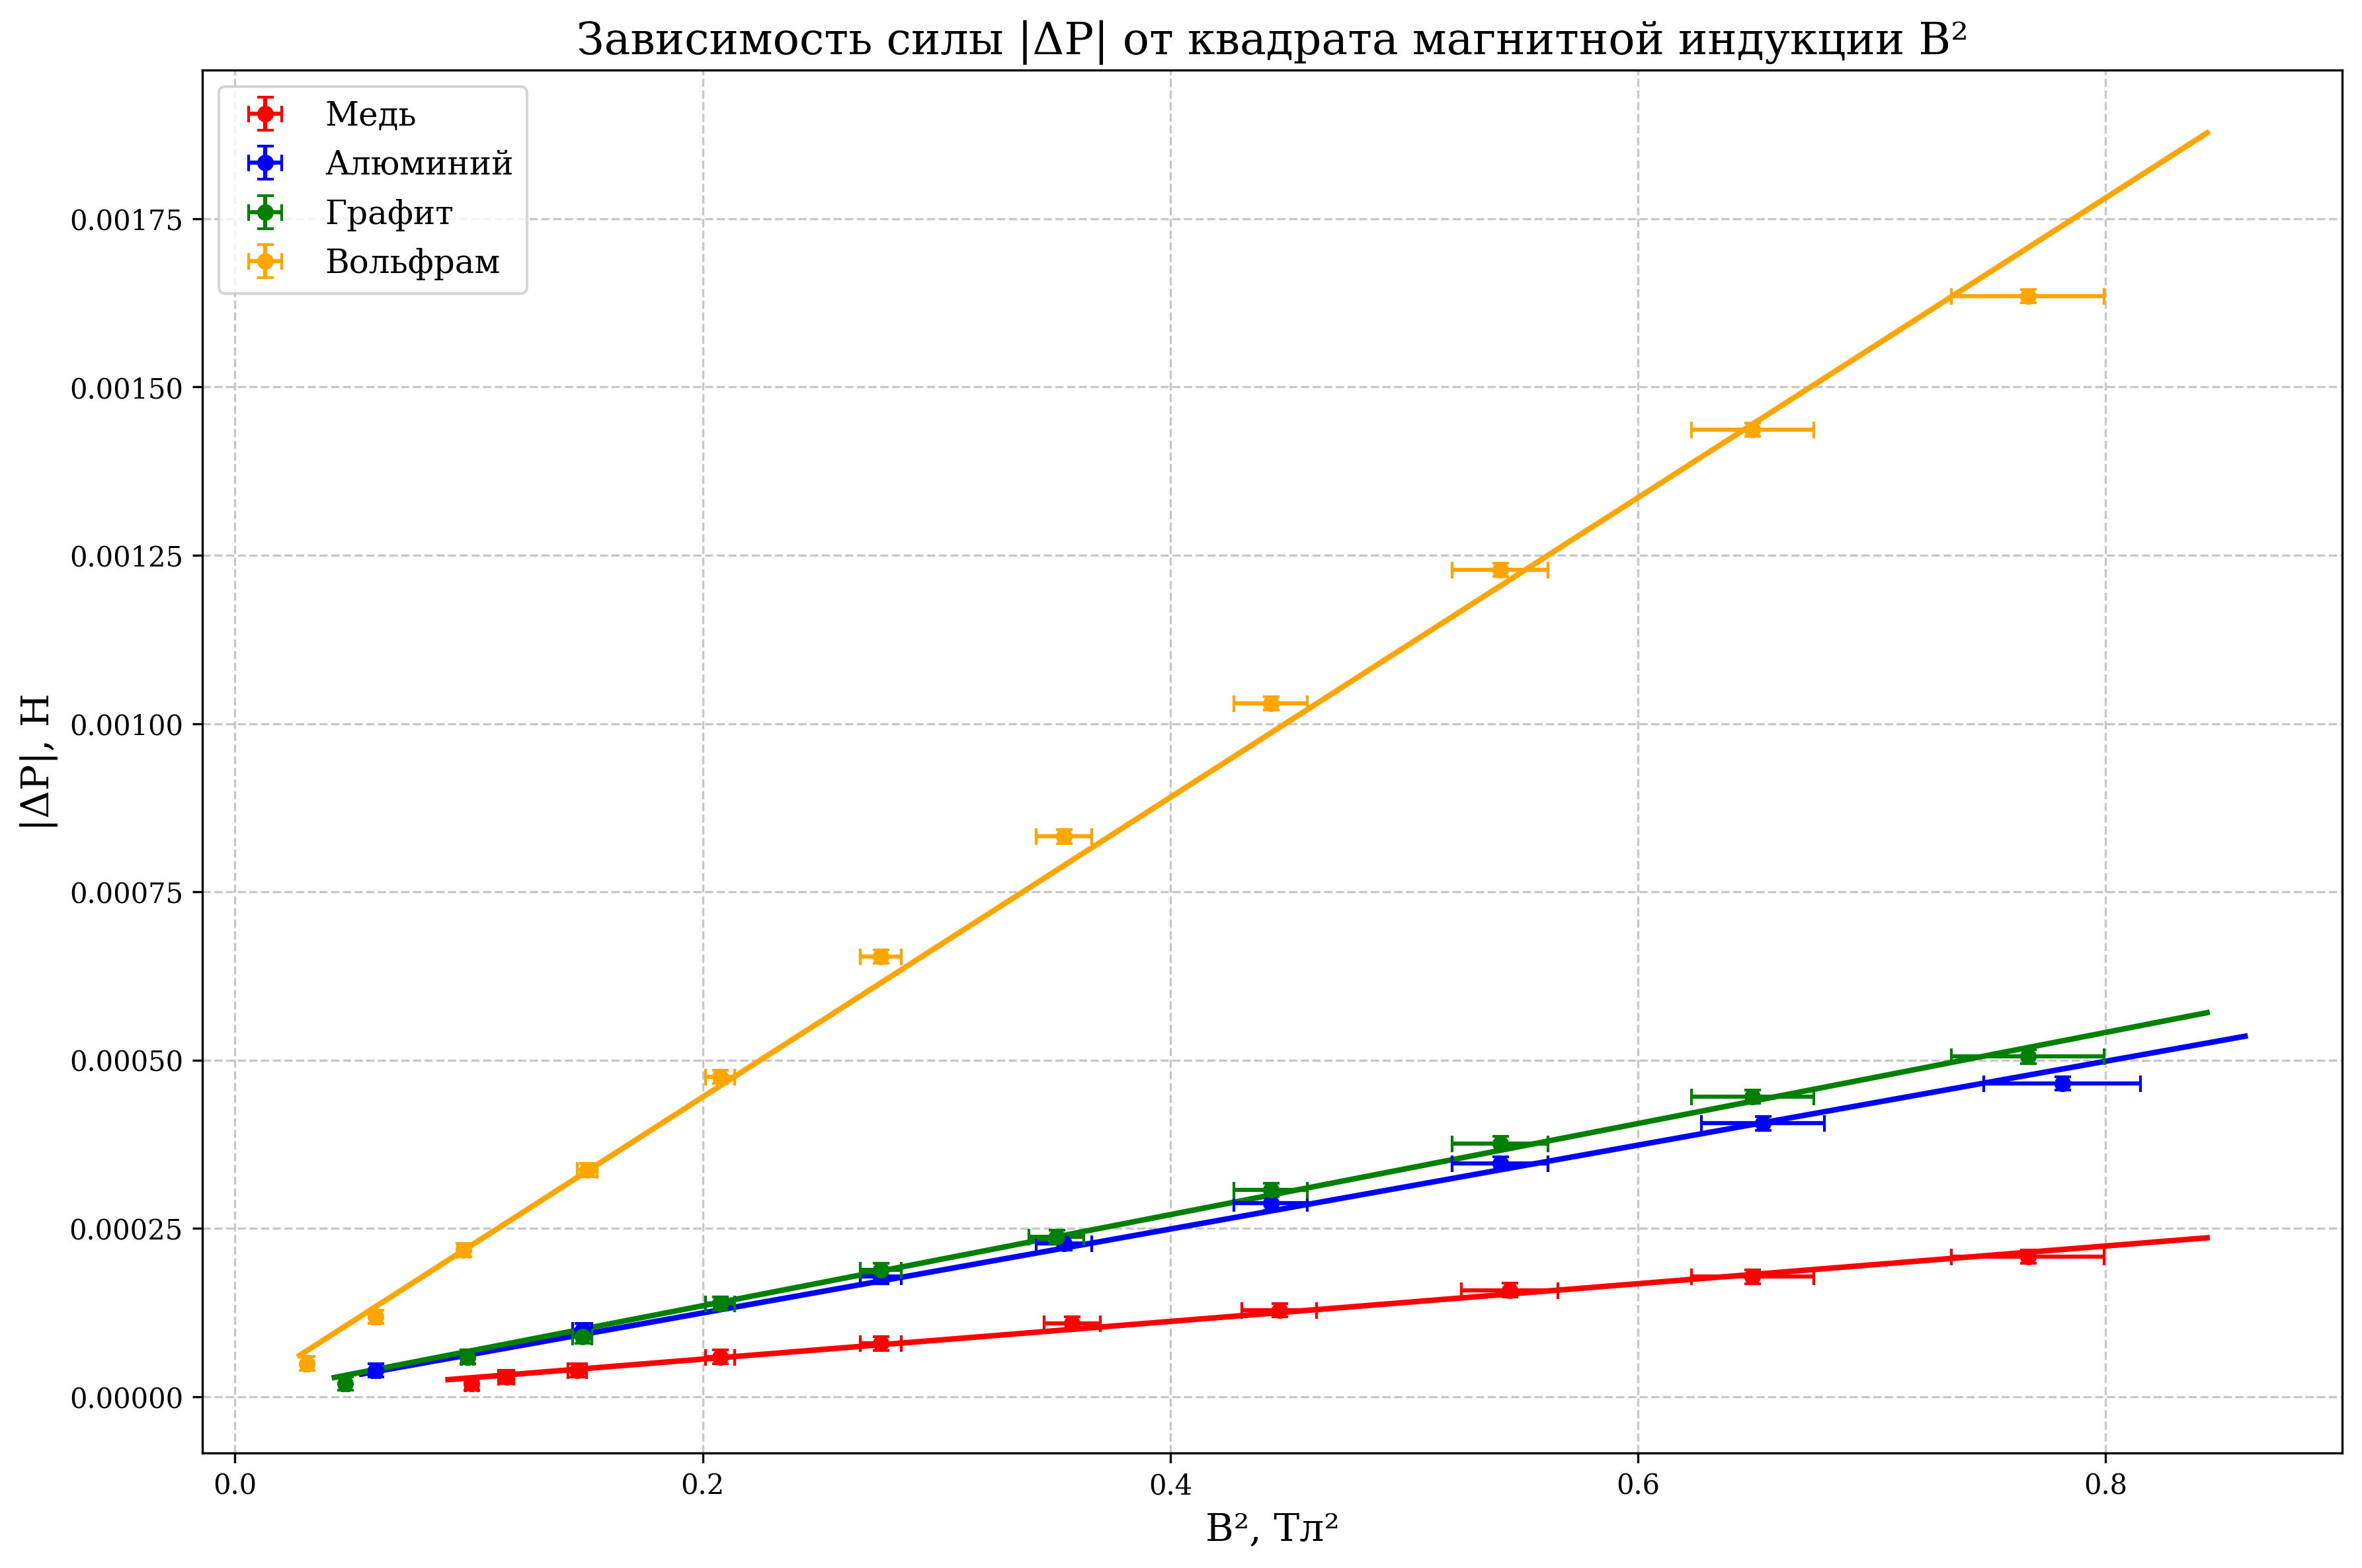
\includegraphics[scale=0.5]{Graphics/all_materials_together.png}
    \caption{График 3. Сравнение всех графиков зависимостей $|\Delta P|(B^2)$ для разных материалов.}
\end{figure}


\item Параметры прямых и рассчитанные по ним восприимчивости $\chi$.
\begin{table}[h!]
    \centering
    \begin{tabular}{|c|c|c|c|}
        \hline
        Материал & $k \pm \sigma_k$, Н/Тл$^2$ & $\chi \pm \sigma_\chi$ & $\varepsilon_\chi$, \% \\ \hline
        Медь & $(-2,80 \pm 0,07) \cdot 10^{-4}$ & $(-8,96 \pm 0,24) \cdot 10^{-6}$ & 2,67 \\ \hline
        Алюминий & $(6,23 \pm 0,07) \cdot 10^{-4}$ & $(1,99 \pm 0,02) \cdot 10^{-5}$ & 1,20 \\ \hline
        Графит & $(-6,77 \pm 0,08) \cdot 10^{-4}$ & $(-6,90 \pm 0,77) \cdot 10^{-5}$ & 1,11 \\ \hline
        Вольфрам & $(2,23 \pm 0,01) \cdot 10^{-3}$ & $(7,12 \pm 0,24) \cdot 10^{-5}$ & 0,34 \\ \hline
    \end{tabular}
    \caption{Результаты измерений магнитной восприимчивости}
    \label{tab:results}
\end{table}
\end{enumerate}

\section{Результаты и обсуждения}

В ходе эксперимента были получены значения магнитной восприимчивости для четырёх материалов методом Гюи. Результаты измерений представлены в сравнительной таблице:

\begin{table}[h!]
    \centering
    \begin{tabular}{|c|c|c|c|}
        \hline
        Материал & $\chi_{\text{эксп}}$, $10^{-6}$ & $\chi_{\text{табл}}$\footnotemark[1], $10^{-6}$ & Отклонение, \% \\ \hline
        Медь & $-8,96 \pm 0,24$ & $-9,63$ & 6,96 \\ \hline
        Алюминий & $19,9 \pm 0,2$ & $21,10$ & 5,69 \\ \hline
        Графит & $-69,0 \pm 0,8$ & $-14,00$ & 392,86 \\ \hline
        Вольфрам & $71,2 \pm 0,2$ & $88,40$ & 19,46 \\ \hline
    \end{tabular}
    \caption{Сравнение экспериментальных и табличных значений магнитной восприимчивости}
    \label{tab:comparison}
\end{table}

\footnotetext[1]{Табличные значения для материалов взяты из следующих источников: медь - \url{https://periodictable.com/Elements/029/data.html}, алюминий -  \url{https://periodictable.com/Elements/013/data.html}, графит - \url{https://periodictable.com/Elements/006/data.html}, вольфрам - \url{https://periodictable.com/Elements/074/data.html}, дата обращения обращения 30.11.2025.}
Анализ полученных результатов показывает:

\begin{itemize}
    \item Для \textbf{меди} и \textbf{алюминия} экспериментальные значения хорошо согласуются с табличными данными. Отклонения составляют 6,96\% и 5,69\% соответственно, что находится в пределах ожидаемой погрешности эксперимента.
    
    \item Для \textbf{вольфрама} наблюдается большее расхождение (19,46\%), что может быть связано с особенностями образца или дополнительными систематическими погрешностями.
    
    \item Наибольшее расхождение отмечено для \textbf{графита} (392,86\%). Столь значительное отклонение может объясняться несколькими факторами:
    \begin{itemize}
        \item Неоднородность структуры графитового образца
        \item Влияние примесей в материале
        \item Особенности ориентации кристаллической решётки графита относительно магнитного поля
        \item Меньший диаметр образца графита (0,56 см) по сравнению с другими материалами
    \end{itemize}
    
    \item Экспериментально подтверждено, что медь и графит являются \textbf{диамагнетиками} ($\chi < 0$), а алюминий и вольфрам --- \textbf{парамагнетиками} ($\chi > 0$).
    
    \item Наименьшую относительную погрешность измерений показал вольфрам (0,34\%), что связано с большими значениями действующей на него силы и, соответственно, лучшей точностью измерений.
\end{itemize}

\section{Выводы}

В ходе лабораторной работы:

\begin{enumerate}
    \item Освоили метод Гюи для измерения магнитной восприимчивости материалов
    \item Провели калибровку электромагнита, установив зависимость $B(I)$
    \item Измерили силы, действующие на образцы в магнитном поле
    \item Определили магнитную восприимчивость четырёх материалов
    \item Экспериментально подтвердили диамагнитные свойства меди и графита, парамагнитные --- алюминия и вольфрама
    \item Получили хорошее согласие с табличными значениями для меди и алюминия
    \item Обнаружили значительное расхождение для графита, требующее дополнительного исследования
\end{enumerate}

Работа демонстрирует работоспособность метода Гюи для определения магнитной восприимчивости и важность контроля чистоты и геометрии образцов для получения точных результатов.
\end{document}